\documentclass{fkssolpub}

\usepackage[czech]{babel}
\usepackage{fontspec}
\usepackage{fkssugar}
\usepackage{amsmath}
\usepackage{graphicx}
\renewcommand{\j}{\mathrm{j}}

\author{Ondřej Sedláček}
\school{Gymnázium Oty Pavla} 
\series{}
\problem{} 

\begin{document}

Pro impedanci vyjádřenou pomocí komplexních čísel platí stejná pravidla pro paralelní a sériové zapojení jako pro odpor, proto:

\[
	\vect{Z}= \frac{\vect{Z_1} \vect{Z_2}}{\vect{Z_1} + \vect{Z_2}} = \frac{\vect{Z_C} {\left(\vect{Z_L} + \vect{Z_{R}}\right)}}{\vect{Z_C} + \vect{Z_L} + \vect{Z_R}}
\]

Teď dosadíme impedanci rezistoru, kapacitoru a cívky:

\[
	\vect{Z}= \frac{\frac{1}{\j \omega C} {\left(\j \omega L + R\right)}}{\frac{1}{\j \omega C} + \j \omega L + R} = \frac{L - \j \frac{R}{\omega}}{R C + \j \left( \omega C L - \frac{1}{\omega} \right)} = \frac{\left(L - \j \frac{R}{\omega}\right)\left(R C - \j \left( \omega C L - \frac{1}{\omega} \right)\right)}{R^2 C^2 + \left( \omega C L - \frac{1}{\omega} \right)^2}
\]

Víme, že pokud bude imaginární část nulová, pak dochází k rezonanci, při kladné imaginární části má obvod induktivní vlastnosti a naopak při záporné imaginární části má obvod kapacitní vlastnosti. Induktivní vlastnosti má obvod tehdy, když:

\[
	\Im \left(\left(L - \j \frac{R}{\omega}\right)\left(R C - \j \left( \omega C L - \frac{1}{\omega} \right)\right)\right) > 0
\]
\[
	- L \left( \omega C L - \frac{1}{\omega} \right) - \frac{R^2 C}{\omega} > 0
\]
\[
	- \omega^2 C L^2 + L - R^2 C > 0
\]
\[
	\omega < \frac{\sqrt{-R^2 + \frac{C}{L}}}{L}
\]

A tedy obvod má induktivní vlastnosti, když:

\[
	f < \frac{\sqrt{-R^2 + \frac{C}{L}}}{L}
\]

Obvod má kapacitní vlastnosti, když:

\[
	f > \frac{\sqrt{-R^2 + \frac{C}{L}}}{L}
\]

A tedy rezonanční frekvence je:

\[
	f_0 = \frac{\sqrt{-R^{2} + \frac{L}{C}}}{2 \pi L}
\]

Teď do $\vect{Z}$ dosadíme hodnoty ze zadání a dostaneme:

\[
	\vect{Z} \doteq 553{,}0715 - 978{,}5475\j
\]

Fázový posun je pak:

\[
	\phi = \arg \vect{Z} \doteq "-1{,}0564 rad" = "299{,}4727^{\circ}"
\]

Pokud fázor napětí je $\vect{U} = U$, pak fázor proudu je:

\[
	\vect{I} = \frac{\vect{U}}{\vect{Z}} = 0{,}00525299 + 0{,}009294 \j
\]

\newpage

Tedy fázorový diagram vypadá nějak následovně (velikosti fázorů neodpovídají skutečným hodnotám, protože by se jinak nevešli do grafu):

\begin{figure}[h!]
	\begin{center}
		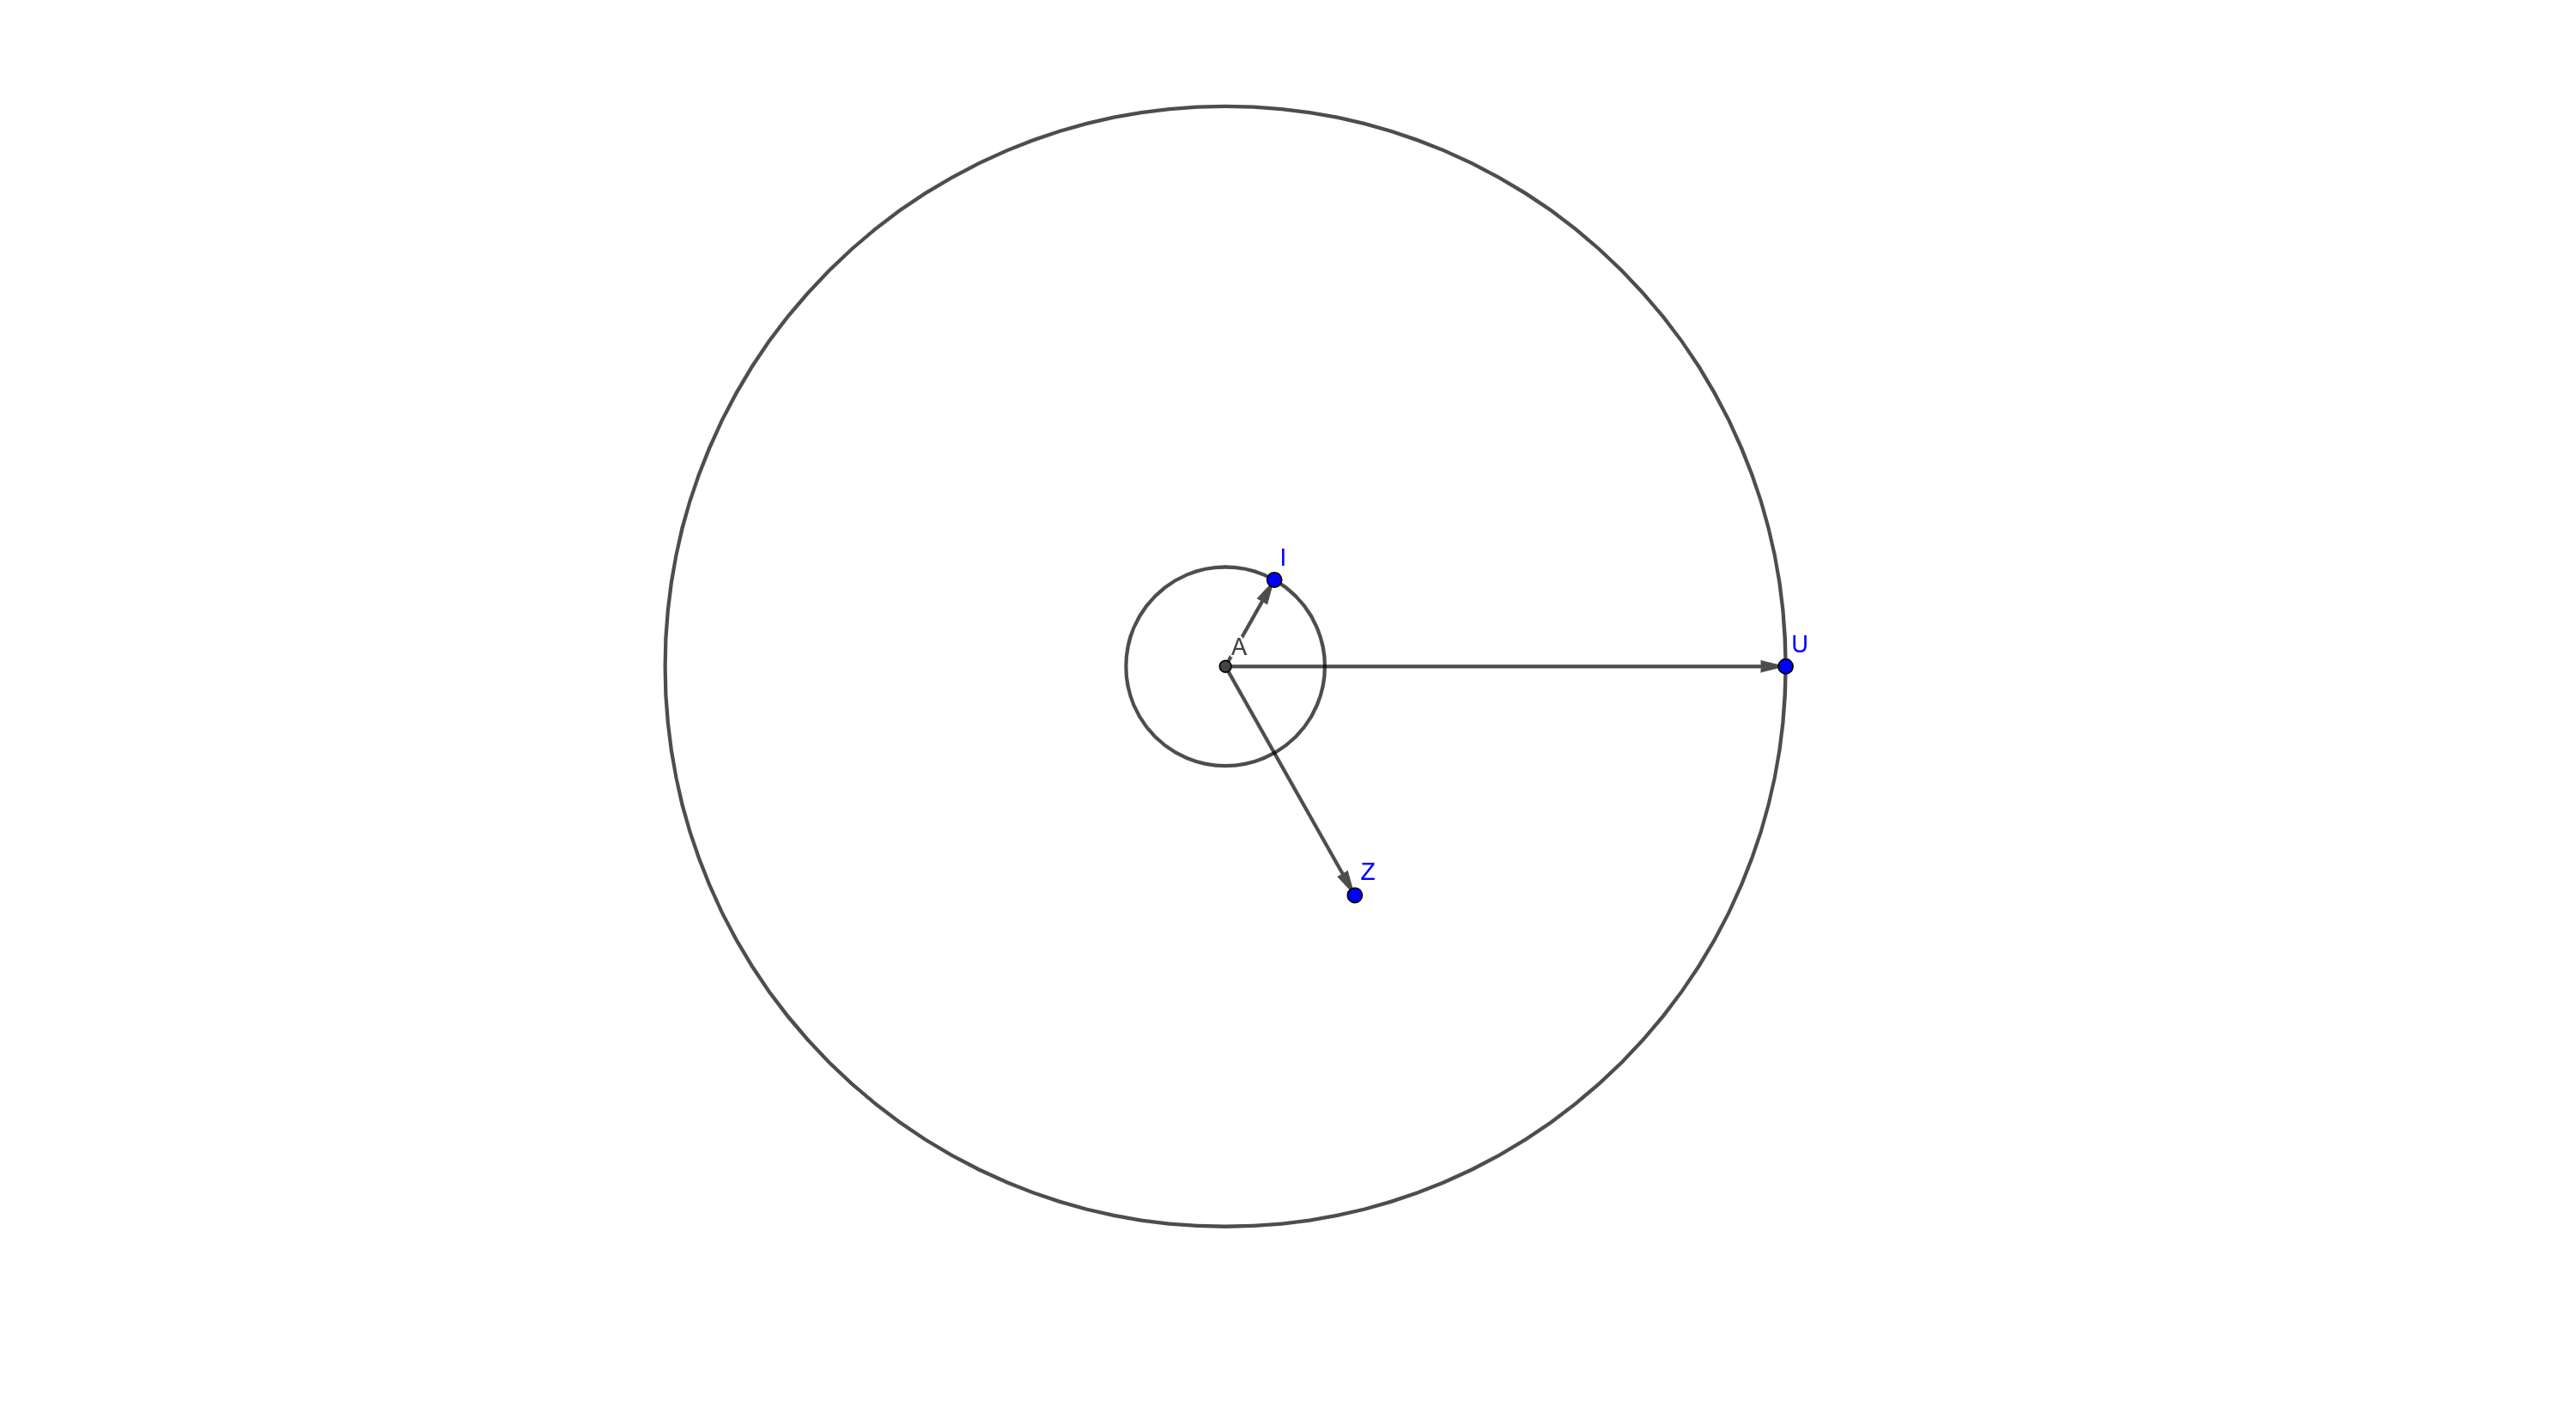
\includegraphics[width=0.95\textwidth]{3-fig.png}
	\end{center}
	\caption{Fázorový diagram}
	\label{fig:1}
\end{figure}


Činný výkon $P$ je pak:

\[
	P = \Re(\vect{U} \cdot \vect{I}) = \Re\left(\frac{\vect{U}^2}{\vect{Z}}\right) = "0{,}06304 W"
\]




\end{document}
